\fancyhead[L]{}
\fancyhead[R]{\textsf{\textbf{MỤC 1.1}}\quad \textsf{Bốn cách biểu diễn một hàm số}\qquad \textbf{\textsf{9}}}

\noindent
\begin{minipage}[t]{0.268\textwidth}
    \vspace*{1.35cm}
    \centering
    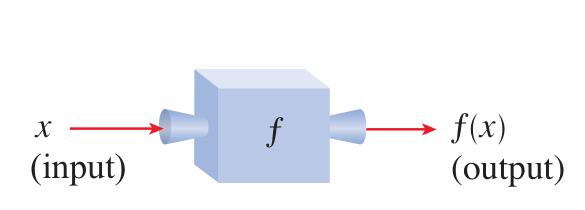
\includegraphics[width=0.95\linewidth]{images/p0044_fig2_clean.png}\\[3pt]
    {\small\textbf{\textsf{HÌNH 2}}}\\[1pt]
    {\fontsize{7.8pt}{9.8pt}\selectfont\color{darkgray} Sơ đồ cỗ máy cho hàm số $f$}

    \vspace{1.6cm}
    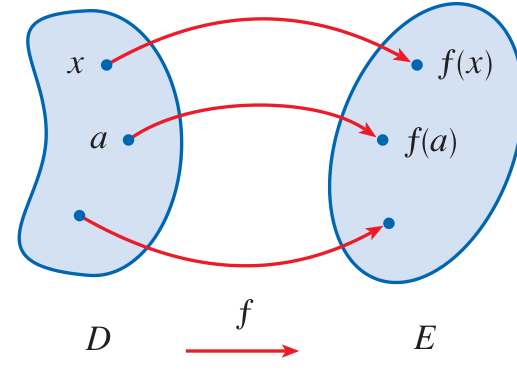
\includegraphics[width=0.88\linewidth]{images/p0044_fig3_clean.png}\\[3pt]
    {\small\textbf{\textsf{HÌNH 3}}}\\[1pt]
    {\fontsize{7.8pt}{9.8pt}\selectfont\color{darkgray} Sơ đồ mũi tên cho $f$}

    \vspace{4.8cm}
    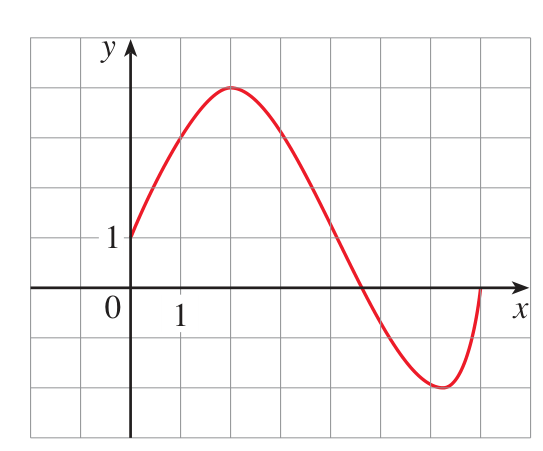
\includegraphics[width=0.92\linewidth]{images/p0044_fig6_clean.png}\\[3pt]
    {\small\textbf{\textsf{HÌNH 6}}}

    \vspace{0.8cm}
    {\fontsize{7.5pt}{9.5pt}\selectfont\color{darkgray}\textit{Ký hiệu các khoảng, đoạn được trình bày trong Phụ lục A.}\par}
\end{minipage}%
\hfill
\begin{minipage}[t]{0.705\textwidth}
    \noindent
    trên toàn bộ tập xác định. Một ký hiệu đại diện cho một số tùy ý thuộc \textit{tập xác định} của hàm số $f$ được gọi là một \textbf{biến độc lập} (\textit{independent variable}). Một ký hiệu đại diện cho một số thuộc \textit{tập giá trị} của $f$ được gọi là một \textbf{biến phụ thuộc} (\textit{dependent variable}). Chẳng hạn, trong Ví dụ A, $r$ là biến độc lập và $A$ là biến phụ thuộc.

    Sẽ rất trực quan nếu ta xem một hàm số như một \textbf{cỗ máy} (xem Hình 2). Nếu $x$ thuộc tập xác định của hàm số $f$, thì khi $x$ đi vào cỗ máy, nó được tiếp nhận như một \textbf{đầu vào} (\textit{input}) và cỗ máy sẽ tạo ra một \textbf{đầu ra} (\textit{output}) là $f(x)$ tuân theo quy tắc xác định của hàm số đó. Do vậy, ta có thể hình dung tập xác định là tập hợp của tất cả các đầu vào khả dĩ, còn tập giá trị là tập hợp của tất cả các đầu ra có thể nhận được. Các hàm được lập trình sẵn trong máy tính cầm tay là những ví dụ điển hình cho mô hình cỗ máy này. Chẳng hạn, nếu bạn nhập một số rồi nhấn phím bình phương, máy tính sẽ hiển thị kết quả đầu ra là bình phương của số vừa nhập.

    Một cách khác để hình dung về hàm số là sử dụng \textbf{sơ đồ mũi tên} (\textit{arrow diagram}) như trong Hình 3. Mỗi mũi tên nối một phần tử thuộc $D$ với một phần tử thuộc $E$. Mũi tên chỉ ra rằng $f(x)$ tương ứng với $x$, $f(a)$ tương ứng với $a$, và cứ tiếp tục như vậy.

    Có lẽ phương pháp hữu ích nhất để trực quan hóa một hàm số là vẽ đồ thị của nó. Nếu $f$ là một hàm số với tập xác định $D$, thì \textbf{đồ thị} (\textit{graph}) của hàm số là tập hợp các cặp có thứ tự:
    \[
    \{ (x, f(x)) \mid x \in D \}
    \]
    (Lưu ý rằng đây chính là các cặp giá trị đầu vào -- đầu ra.) Nói cách khác, đồ thị của $f$ bao gồm tất cả các điểm $(x, y)$ trên mặt phẳng tọa độ sao cho $y = f(x)$ và $x$ thuộc tập xác định của $f$.

    Đồ thị của một hàm số $f$ đem lại cho ta một bức tranh trực quan hữu ích về hành vi hay ``tiến trình biến thiên'' của hàm số đó. Do tọa độ $y$ của bất kỳ điểm $(x, y)$ nào trên đồ thị đều là $y = f(x)$, ta có thể đọc giá trị của $f(x)$ từ đồ thị bằng chính độ cao của đồ thị nằm phía trên điểm $x$ (xem Hình 4). Đồ thị của $f$ cũng cho phép ta hình dung trực quan tập xác định của $f$ trên trục hoành ($x$) và tập giá trị của nó trên trục tung ($y$) như minh họa trong Hình 5.

    \vspace{4pt}
    \noindent
    \begin{minipage}[t]{0.48\linewidth}
        \centering
        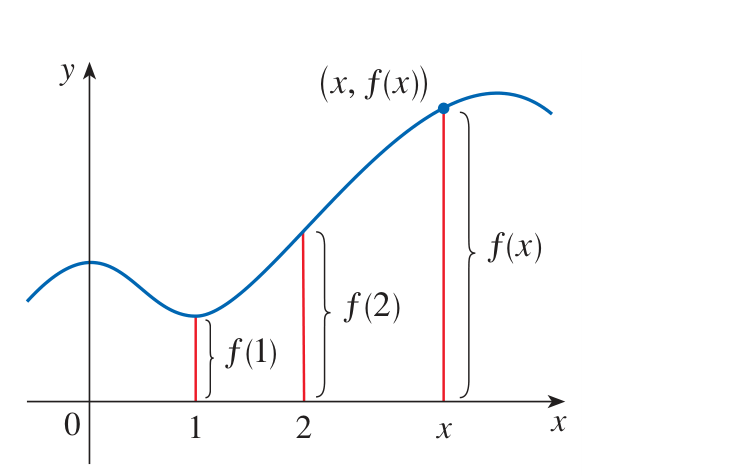
\includegraphics[height=3.2cm,keepaspectratio]{images/p0044_fig4_clean.png}\\[2pt]
        {\small\textbf{\textsf{HÌNH 4}}}
    \end{minipage}\hfill
    \begin{minipage}[t]{0.48\linewidth}
        \centering
        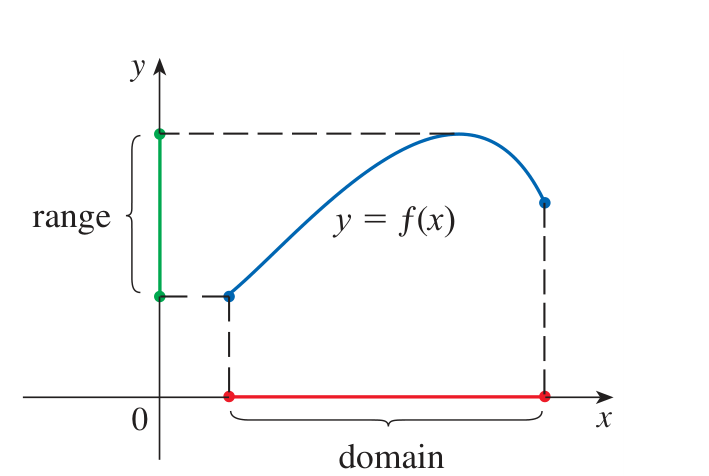
\includegraphics[height=3.2cm,keepaspectratio]{images/p0044_fig5_clean.png}\\[2pt]
        {\small\textbf{\textsf{HÌNH 5}}}
    \end{minipage}

    \vspace{6pt}
    \noindent{\large\textbf{\textsf{\color{stewartcyan}VÍ DỤ 1}}}\quad Đồ thị của một hàm số $f$ được cho trong Hình 6.
    \begin{enumerate}[label=(\alph*), itemsep=0.5pt, topsep=1pt, leftmargin=1.5em]
        \item Tìm các giá trị của $f(1)$ và $f(5)$.
        \item Tập xác định và tập giá trị của $f$ là gì?
    \end{enumerate}

    \noindent{\textbf{\textsf{\color{stewartcyan}LỜI GIẢI}}}

    \textbf{(a)} Từ Hình 6, ta thấy điểm $(1, 3)$ nằm trên đồ thị của $f$, do đó giá trị của $f$ tại $1$ là $f(1) = 3$. (Nói cách khác, điểm trên đồ thị nằm thẳng phía trên $x = 1$ cách trục $x$ một khoảng bằng $3$ đơn vị.)

    Khi $x = 5$, đồ thị nằm bên dưới trục $x$ khoảng $0{,}7$ đơn vị, vì vậy ta ước lượng được $f(5) \approx -0{,}7$.

    \textbf{(b)} Ta thấy $f(x)$ được xác định khi $0 \le x \le 7$, do đó tập xác định của $f$ là đoạn đóng $[0, 7]$. Lưu ý rằng $f$ nhận tất cả các giá trị từ $-2$ đến $4$, vì thế tập giá trị của $f$ là:
    \[
    \{ y \mid -2 \le y \le 4 \} = [-2, 4] \tag*{\color{stewartcyan}$\blacksquare$}
    \]
\end{minipage}